% Multi-panel figure generated by plot_experiment2_width_ratio_rf.py --runs exp2_real.
% Requires \usepackage{graphicx} and \usepackage{subcaption}. Paths are relative
% to the repo root (Figs/...); adjust \graphicspath or the paths below.
% Include with: % Multi-panel figure generated by plot_experiment2_width_ratio_rf.py --runs exp2_real.
% Requires \usepackage{graphicx} and \usepackage{subcaption}. Paths are relative
% to the repo root (Figs/...); adjust \graphicspath or the paths below.
% Include with: % Multi-panel figure generated by plot_experiment2_width_ratio_rf.py --runs exp2_real.
% Requires \usepackage{graphicx} and \usepackage{subcaption}. Paths are relative
% to the repo root (Figs/...); adjust \graphicspath or the paths below.
% Include with: % Multi-panel figure generated by plot_experiment2_width_ratio_rf.py --runs exp2_real.
% Requires \usepackage{graphicx} and \usepackage{subcaption}. Paths are relative
% to the repo root (Figs/...); adjust \graphicspath or the paths below.
% Include with: \input{width_ratio_rf_exp2_real_figure}
\begin{figure}[htbp]
\centering
\begin{subfigure}[t]{0.48\linewidth}
  \centering
  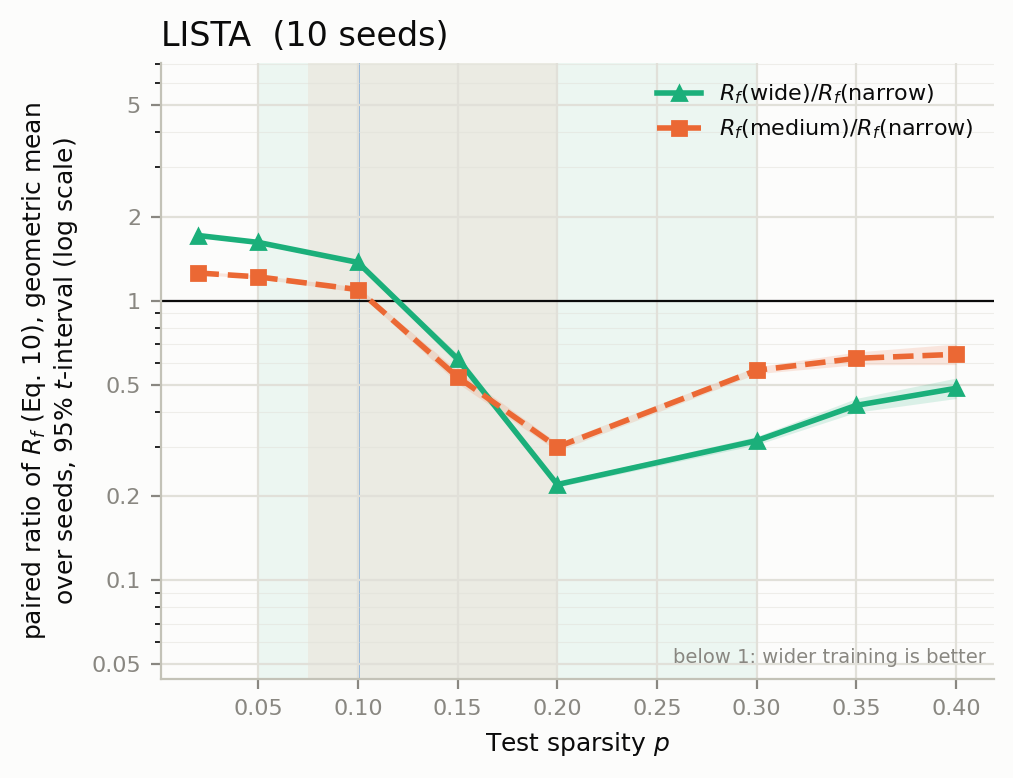
\includegraphics[width=\linewidth]{Figs/exp2_real/width_ratio_rf_exp2_real_lista.png}
  \caption{LISTA}
  \label{fig:width-ratio-rf-exp2-real-lista}
\end{subfigure}\hfill
\begin{subfigure}[t]{0.48\linewidth}
  \centering
  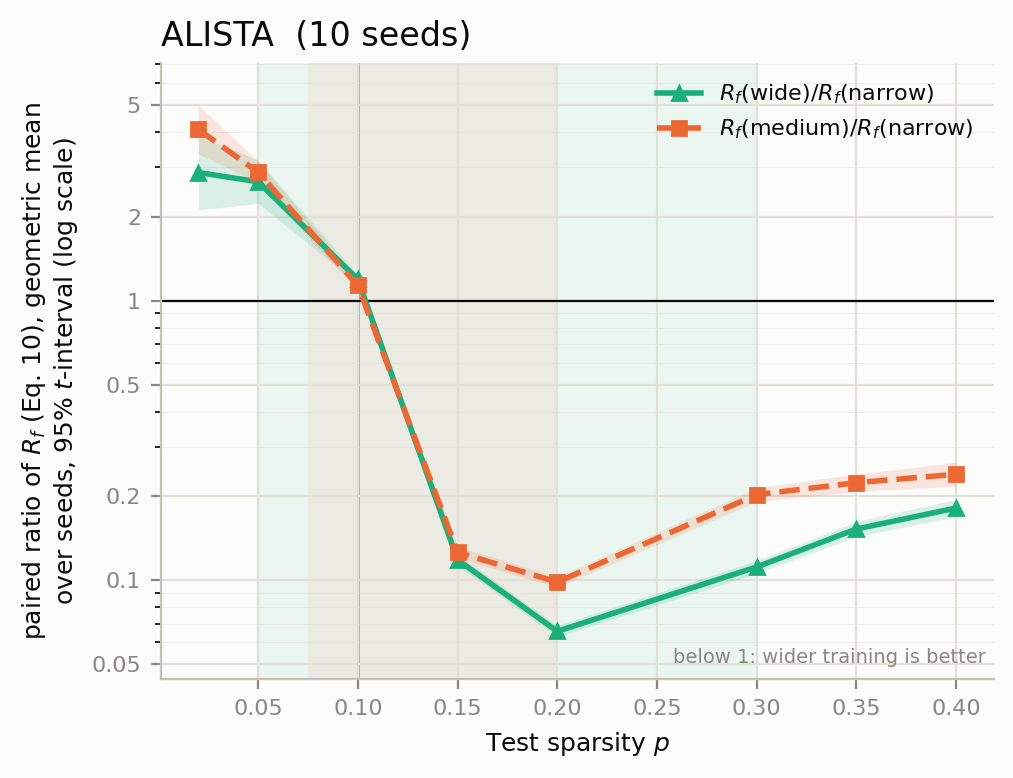
\includegraphics[width=\linewidth]{Figs/exp2_real/width_ratio_rf_exp2_real_alista.png}
  \caption{ALISTA}
  \label{fig:width-ratio-rf-exp2-real-alista}
\end{subfigure}
\caption{Effect of the training-sparsity width on the modified relative loss $R_f$ (Eq.~10), $(m,n) = (210, 300)$, SNR 40 dB, uncentred widths. For each test sparsity $p$ the ratio $R_f(\text{wide}) / R_f(\text{narrow})$ and $R_f(\text{medium}) / R_f(\text{narrow})$ is computed per seed (same dictionary, test instances and $x_0$ for every width) and summarised as the geometric mean over seeds with a 95\% $t$-interval on $\log R_f$; below 1 means the wider training distribution is better on the objective. Shaded bands are the medium and wide training supports, the vertical line the fixed narrow training point. Both panels share the y-axis.}
\label{fig:width-ratio-rf-exp2-real}
\end{figure}

\begin{figure}[htbp]
\centering
\begin{subfigure}[t]{0.48\linewidth}
  \centering
  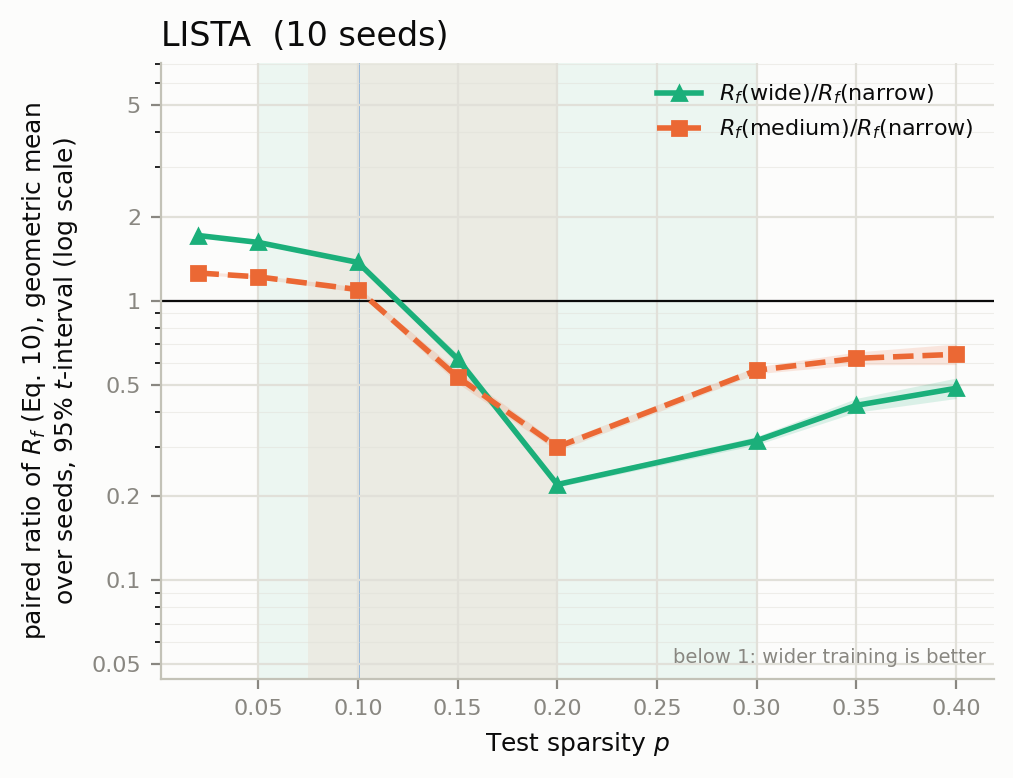
\includegraphics[width=\linewidth]{Figs/exp2_real/width_ratio_rf_exp2_real_lista.png}
  \caption{LISTA}
  \label{fig:width-ratio-rf-exp2-real-lista}
\end{subfigure}\hfill
\begin{subfigure}[t]{0.48\linewidth}
  \centering
  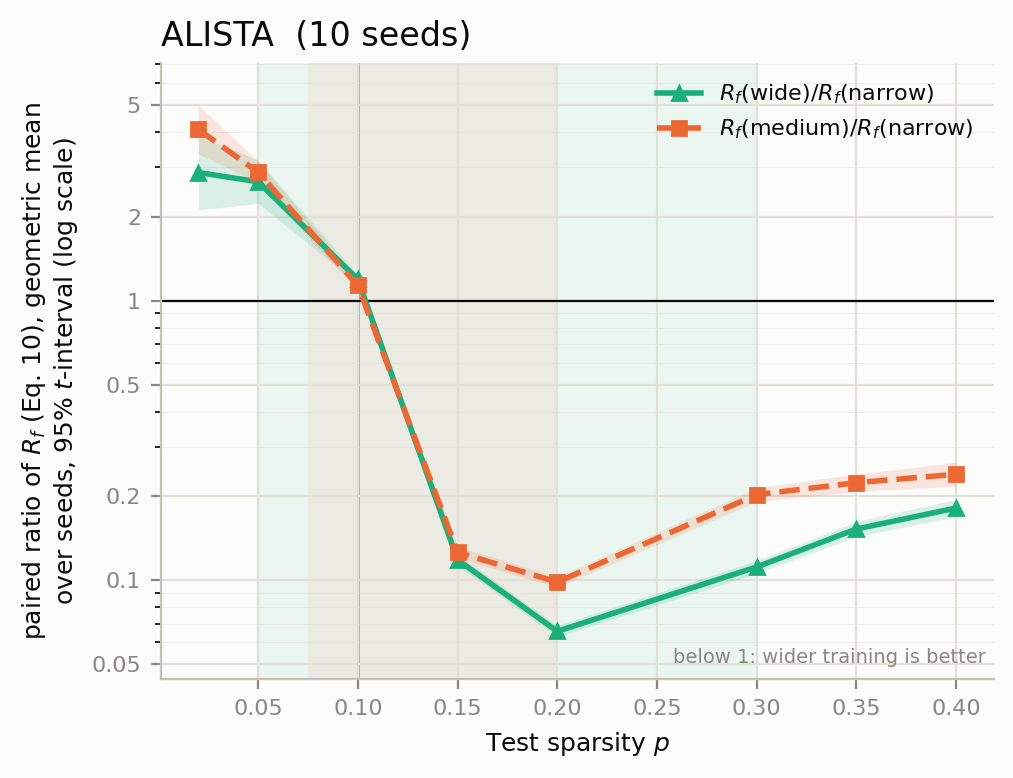
\includegraphics[width=\linewidth]{Figs/exp2_real/width_ratio_rf_exp2_real_alista.png}
  \caption{ALISTA}
  \label{fig:width-ratio-rf-exp2-real-alista}
\end{subfigure}
\caption{Effect of the training-sparsity width on the modified relative loss $R_f$ (Eq.~10), $(m,n) = (210, 300)$, SNR 40 dB, uncentred widths. For each test sparsity $p$ the ratio $R_f(\text{wide}) / R_f(\text{narrow})$ and $R_f(\text{medium}) / R_f(\text{narrow})$ is computed per seed (same dictionary, test instances and $x_0$ for every width) and summarised as the geometric mean over seeds with a 95\% $t$-interval on $\log R_f$; below 1 means the wider training distribution is better on the objective. Shaded bands are the medium and wide training supports, the vertical line the fixed narrow training point. Both panels share the y-axis.}
\label{fig:width-ratio-rf-exp2-real}
\end{figure}

\begin{figure}[htbp]
\centering
\begin{subfigure}[t]{0.48\linewidth}
  \centering
  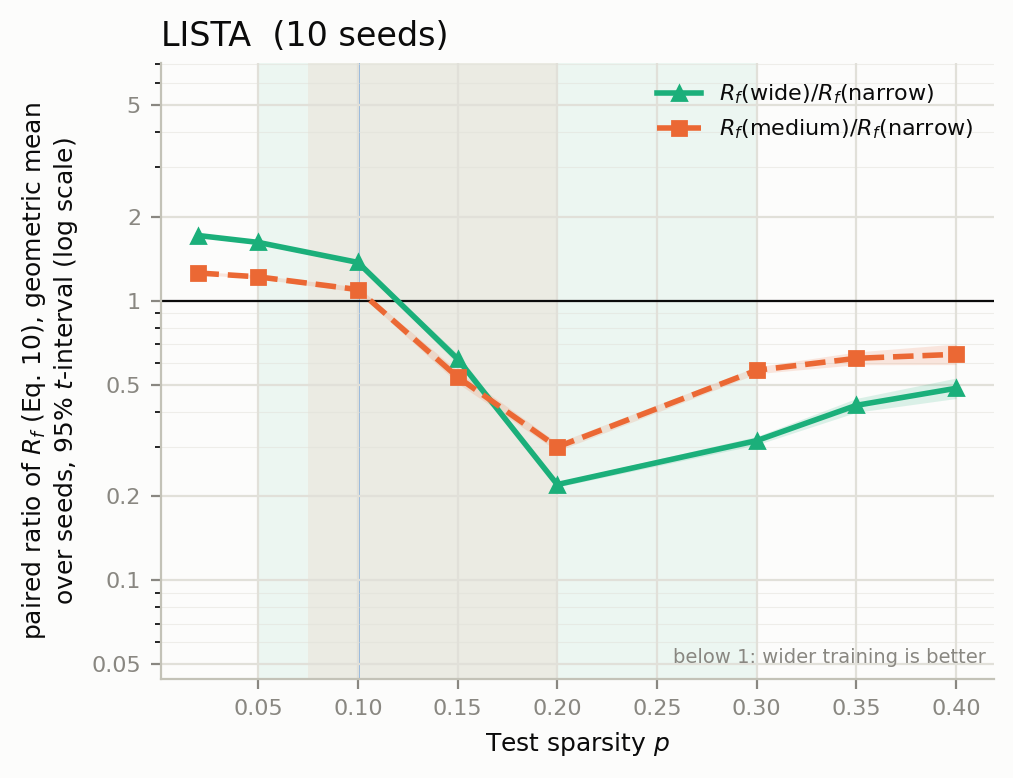
\includegraphics[width=\linewidth]{Figs/exp2_real/width_ratio_rf_exp2_real_lista.png}
  \caption{LISTA}
  \label{fig:width-ratio-rf-exp2-real-lista}
\end{subfigure}\hfill
\begin{subfigure}[t]{0.48\linewidth}
  \centering
  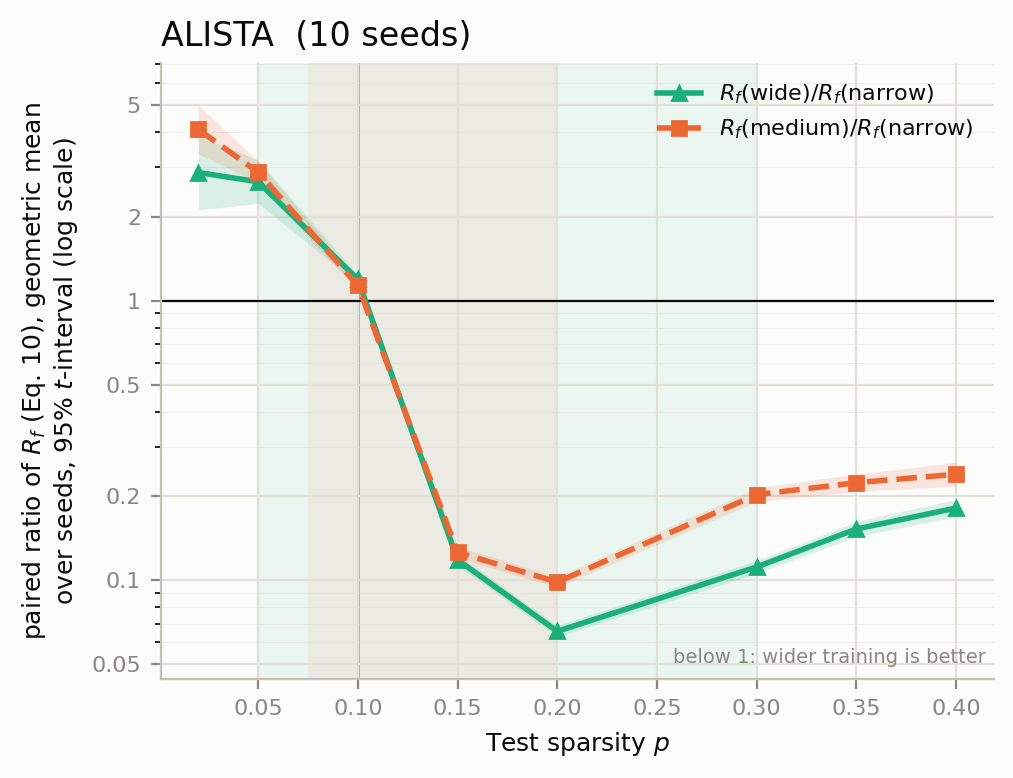
\includegraphics[width=\linewidth]{Figs/exp2_real/width_ratio_rf_exp2_real_alista.png}
  \caption{ALISTA}
  \label{fig:width-ratio-rf-exp2-real-alista}
\end{subfigure}
\caption{Effect of the training-sparsity width on the modified relative loss $R_f$ (Eq.~10), $(m,n) = (210, 300)$, SNR 40 dB, uncentred widths. For each test sparsity $p$ the ratio $R_f(\text{wide}) / R_f(\text{narrow})$ and $R_f(\text{medium}) / R_f(\text{narrow})$ is computed per seed (same dictionary, test instances and $x_0$ for every width) and summarised as the geometric mean over seeds with a 95\% $t$-interval on $\log R_f$; below 1 means the wider training distribution is better on the objective. Shaded bands are the medium and wide training supports, the vertical line the fixed narrow training point. Both panels share the y-axis.}
\label{fig:width-ratio-rf-exp2-real}
\end{figure}

\begin{figure}[htbp]
\centering
\begin{subfigure}[t]{0.48\linewidth}
  \centering
  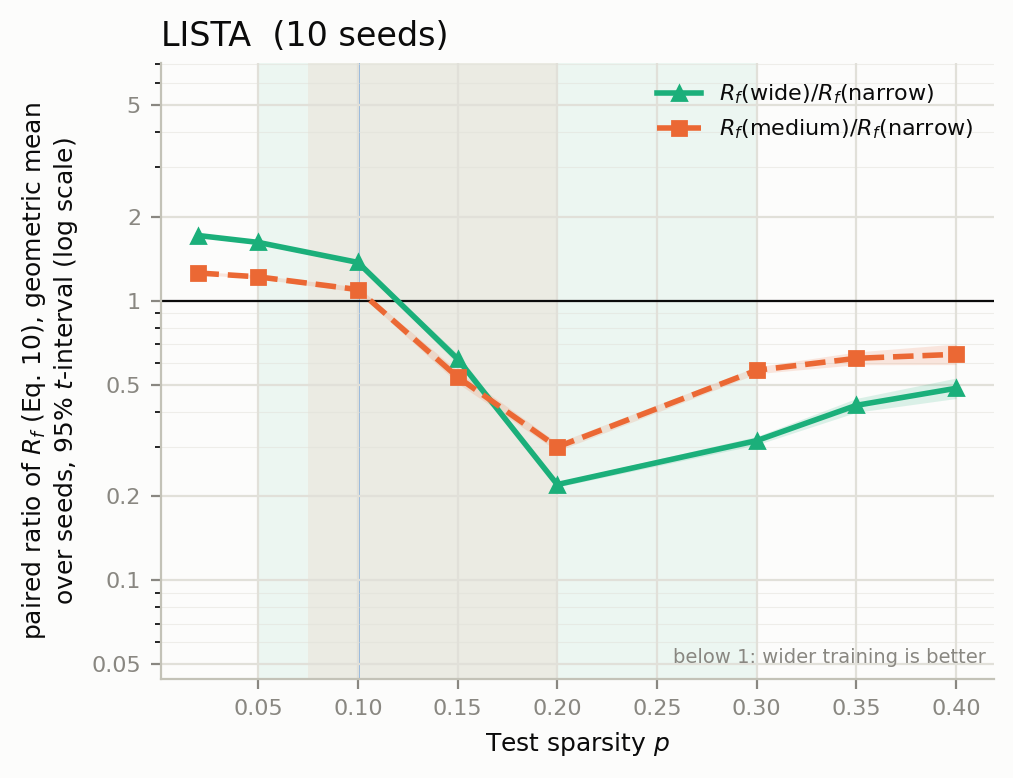
\includegraphics[width=\linewidth]{Figs/exp2_real/width_ratio_rf_exp2_real_lista.png}
  \caption{LISTA}
  \label{fig:width-ratio-rf-exp2-real-lista}
\end{subfigure}\hfill
\begin{subfigure}[t]{0.48\linewidth}
  \centering
  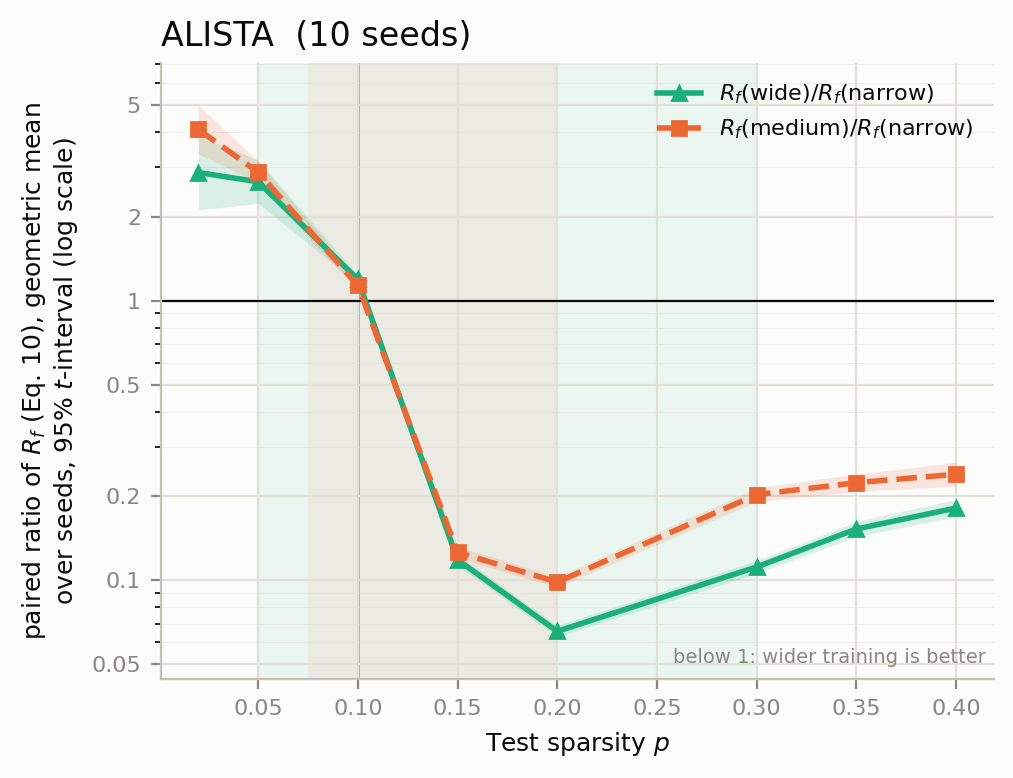
\includegraphics[width=\linewidth]{Figs/exp2_real/width_ratio_rf_exp2_real_alista.png}
  \caption{ALISTA}
  \label{fig:width-ratio-rf-exp2-real-alista}
\end{subfigure}
\caption{Effect of the training-sparsity width on the modified relative loss $R_f$ (Eq.~10), $(m,n) = (210, 300)$, SNR 40 dB, uncentred widths. For each test sparsity $p$ the ratio $R_f(\text{wide}) / R_f(\text{narrow})$ and $R_f(\text{medium}) / R_f(\text{narrow})$ is computed per seed (same dictionary, test instances and $x_0$ for every width) and summarised as the geometric mean over seeds with a 95\% $t$-interval on $\log R_f$; below 1 means the wider training distribution is better on the objective. Shaded bands are the medium and wide training supports, the vertical line the fixed narrow training point. Both panels share the y-axis.}
\label{fig:width-ratio-rf-exp2-real}
\end{figure}
